%%%%%%%%%%%%%%%%%%%%%%%%%%%%%%%%%%%%%%%%%%%%%%%%%%%%%%%%%%%%%%%%%%%%%%%%%%%%%%%%
%2345678901234567890123456789012345678901234567890123456789012345678901234567890
%        1         2         3         4         5         6         7         8

\documentclass[letterpaper, 10 pt, conference]{ieeeconf}  % Comment this line out
                                                          % if you need a4paper
%\documentclass[a4paper, 10pt, conference]{ieeeconf}      % Use this line for a4
                                                          % paper

\IEEEoverridecommandlockouts                              % This command is only
                                                          % needed if you want to
                                                          % use the \thanks command
\overrideIEEEmargins
% See the \addtolength command later in the file to balance the column lengths
% on the last page of the document



\usepackage{tikz}
\usepackage{flushend}
\usepackage[algoruled,vlined,linesnumbered]{algorithm2e}
\usepackage{graphicx}        % standard LaTeX graphics tool
\usepackage[TABTOPCAP]{subfigure}
\usepackage{enumerate}
\usepackage{fancybox}
%added two new packages
\usepackage{amssymb}
\usepackage{amsmath}
\usepackage{lettrine}

\usepackage[linkbordercolor={1 1 1},citebordercolor={1 1
  1},urlbordercolor={0.0 0.0
  0.0},urlcolor=blue,colorlinks=true,linkcolor=black,citecolor=black]{hyperref}
\usepackage[squaren]{SIunits}
\usetikzlibrary{matrix,calc,shapes}
\usepackage{fancyhdr}

\definecolor{nodecolor}{RGB}{238,232,170} % light goldenrod
\definecolor{bgcolor}{rgb}{0.9,0.9,1.0} % light blue
\definecolor{sectcolor}{rgb}{0.0,0.0,0.5} % dark blue




% The following packages can be found on http:\\www.ctan.org
%\usepackage{graphics} % for pdf, bitmapped graphics files
%\usepackage{epsfig} % for postscript graphics files
%\usepackage{mathptmx} % assumes new font selection scheme installed
%\usepackage{times} % assumes new font selection scheme installed
%\usepackage{amsmath} % assumes amsmath package installed
%\usepackage{amssymb}  % assumes amsmath package installed

\title{\LARGE \bf
Multi-Process Approach to Reliable Control of Humanoid Robots
}

\author{Daniel M. Lofaro$^{1}$, Neil Dantam$^{2}$, Michael Grey$^{2}$, Mike Stilman$^{3}$, and Paul Oh$^{4}$% <-this % stops a space
\thanks{*This work was supported in part by the Defense Advanced Research Projects Agency (DARPA) award #N65236-12-1-1005 for the DARPA Robotics Challenge.}% <-this % stops a space
\thanks{$^{1}$D. Lofaro is a Ph.D Candidate of the Electrical and Computer Engineering Department,
        Drexel University, 3141 Chestnut St, Philadelphia PA, USA
        {\tt\small dan at danlofaro.com}}%
\thanks{$^{2}$N. Dantam and M. Grey are Ph.D students with the Department of Computer Science, Georgia Institute of Technology,
        Atlanta GA, USA
        {\tt\small ntd at gatech.edu and mxgrey at gatech.edu}}%
\thanks{$^{3}$M. Stilman is with Faculty of Department of Computer Science, Georgia Institute of Technology,
        Atlanta GA, USA
        {\tt\small mstilman at cc.gatech.edu}}%
\thanks{$^{4}$P. Oh is with Faculty of Mechanical Engineering,
        Drexel University, 3141 Chestnut St, Philadelphia PA, USA
        {\tt\small paul at coe.drexel.edu}}%
}


\begin{document}



\maketitle
\thispagestyle{empty}
\pagestyle{empty}


%%%%%%%%%%%%%%%%%%%%%%%%%%%%%%%%%%%%%%%%%%%%%%%%%%%%%%%%%%%%%%%%%%%%%%%%%%%%%%%%
\begin{abstract}

\end{abstract}
%%%%%%%%%%%%%%%%%%%%%%%%%%%%%%%%%%%%%%%%%%%%%%%%%%%%%%%%%%%%%%%%%%%%%%%%%%%%%%%%

%\subsubsection{Hubo2 Plus}
The Hubo2+ is a $1.3\meter$ (4' 3'') tall, 42 $kg$ (93 $lb$) full-size
humanoid robot.  The Hubo series was designed and constructed by the
Korean Advanced Institute of Science and Technology (KAIST) and
spinoff Rainbow Inc. \cite{hubofirst}.  It has 38 degree of freedom:
six per arm and leg, five per hand, three in the neck, and one in the
waist.  Sensors include three-axis force-torque sensors in the wrists
and ankles, accelerometers in the feet, and an inertial measurement
unit (IMU).  The sensors and embedded motor controllers are connected
via a Controller Area Network to a pair of Intel Atom PC104+ PCs
running a GNU/Linux distribution.



% The reference commands for
% all of the joints are sent from the primary control computer (x86) to
% the individual motor controllers via two Controller Area Network (CAN)
% buses.  This is the same communications bus found in most modern motor
% vehicles.  There are currently eight Hubo's functioning in the United
% States as of December 2012.  Four reside at Drexel University and one
% at Georgia Tech, Purdue, Ohio State and MIT.  Jaemi Hubo is the oldest
% of the Hubos in America and has been at the Drexel Autonomous Systems
% Lab\footnote{Drexel Autonomous Systems Lab:
%   http://dasl.mem.drexel.edu/} (DASL) since 2008 \cite{jaemiHuboSRM}.
% Fig.~\ref{fig:hubo} shows the major dimensions of Hubo.

% \begin{figure}[thpb]
%   \centering
% 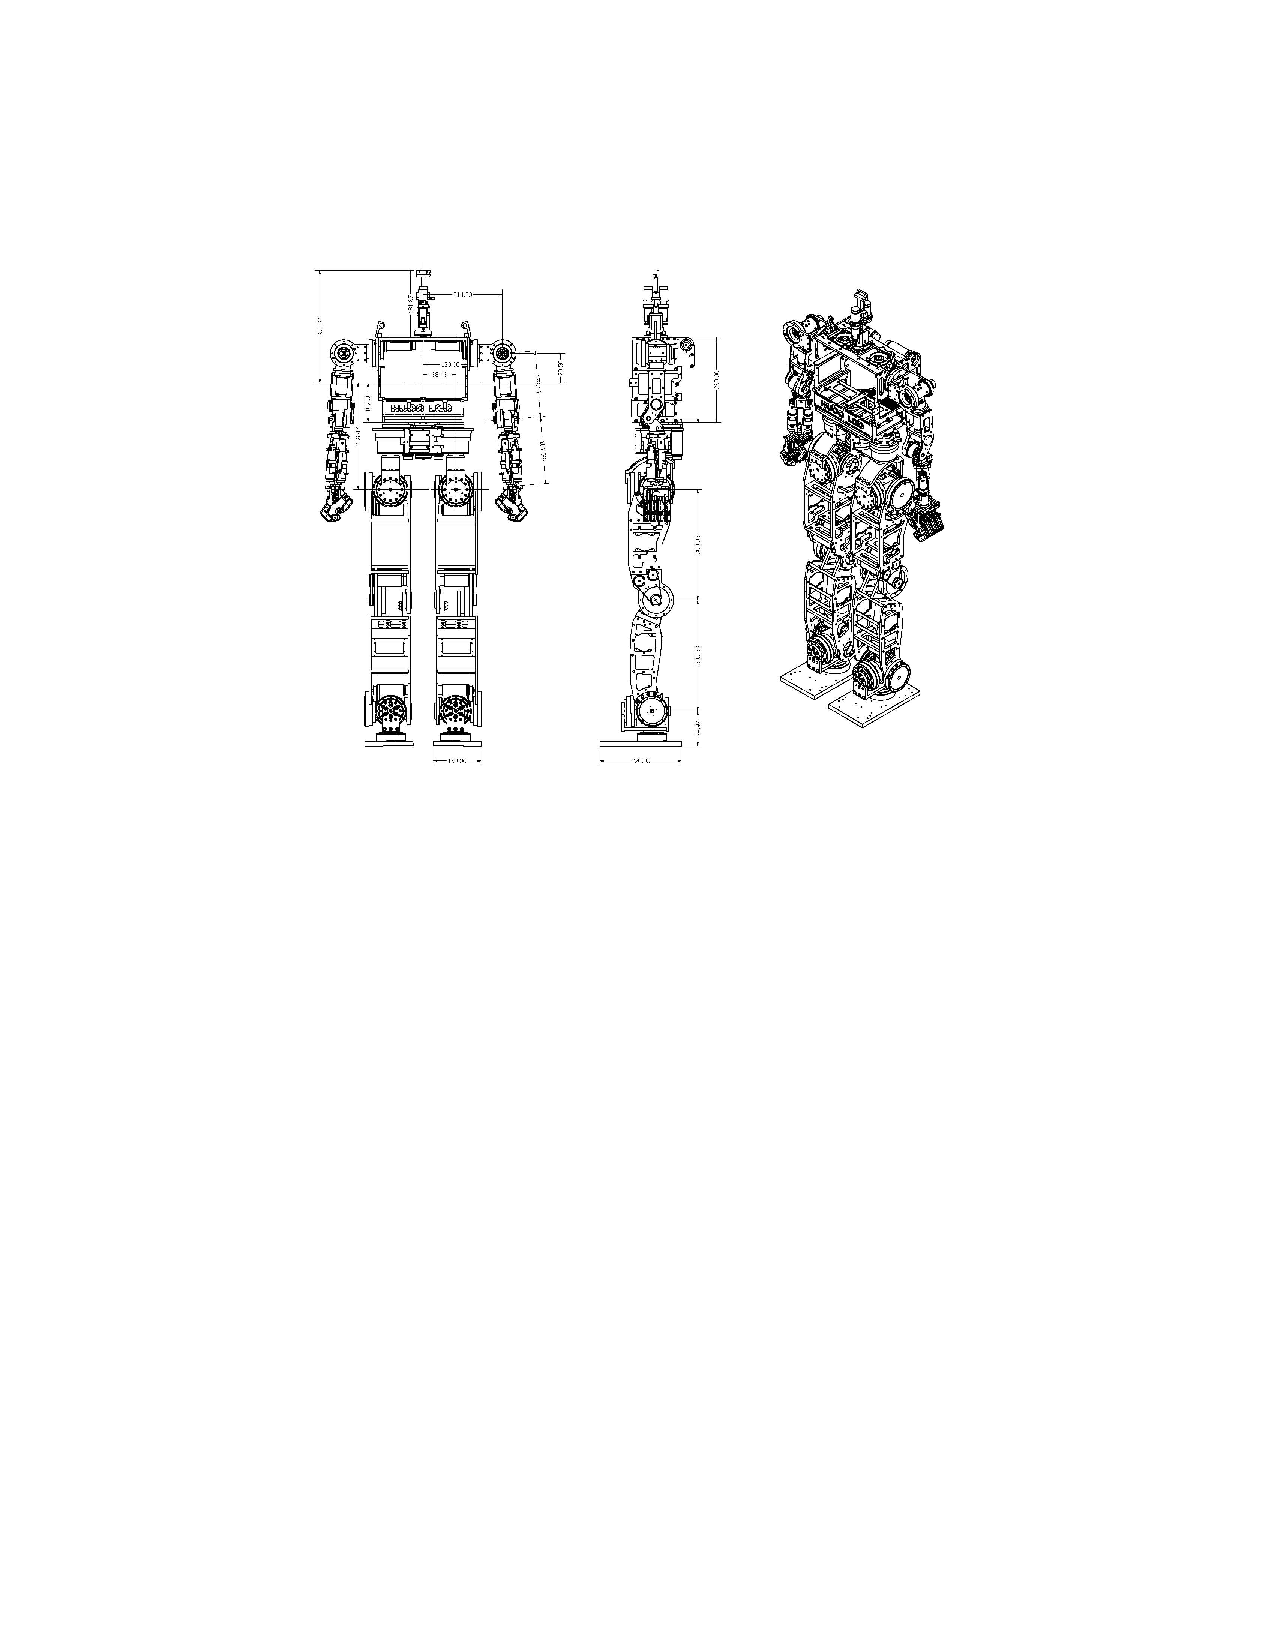
\includegraphics[width=1.0\columnwidth]{./pix/huboSkel.pdf}
%   \caption{Hubo2 Plus platform: 38 DOF, 130 $cm$ tall full-size humanoid robot weighing 37 $kg$.}
%   \label{fig:hubo}
% \end{figure}

% All joints of the major joints are high gain PID position
% controlled with the exception of the fingers.  The fingers are
% open-loop PWM controlled.
% The sensing capability consists of a three
% axis force-torque (FT) sensor on each leg between the end of the ankle
% and the foot as well as between the arm where it connects to the hand.
% Additionally it has an inertial measurement unit (IMU) at the center
% of mass and accelerometers on each foot.

%%% Local Variables:
%%% mode: latex
%%% TeX-master: "ach"
%%% End:


%\section{Hubo-Ach: Linux on Hubo}

The Hubo2+ is a $1.3\meter$ tall, $42 \kilo\gram$ full-size humanoid
robot, produced by the Korean Advanced Institute of Science and
Technology (KAIST) and spinoff company Rainbow Inc. \cite{hubofirst}.
It has 38 DOF: six per arm and leg, five per hand, three in the neck,
and one in the waist.  Sensors include three-axis force-torque sensors
in the wrists and ankles, accelerometers in the feet, and an inertial
measurement unit (IMU).  The sensors and embedded motor controllers
are connected via a Controller Area Network to a pair of Intel Atom
PC104+ PCs.

% \begin{figure*}[thpb]
%   \centering
% 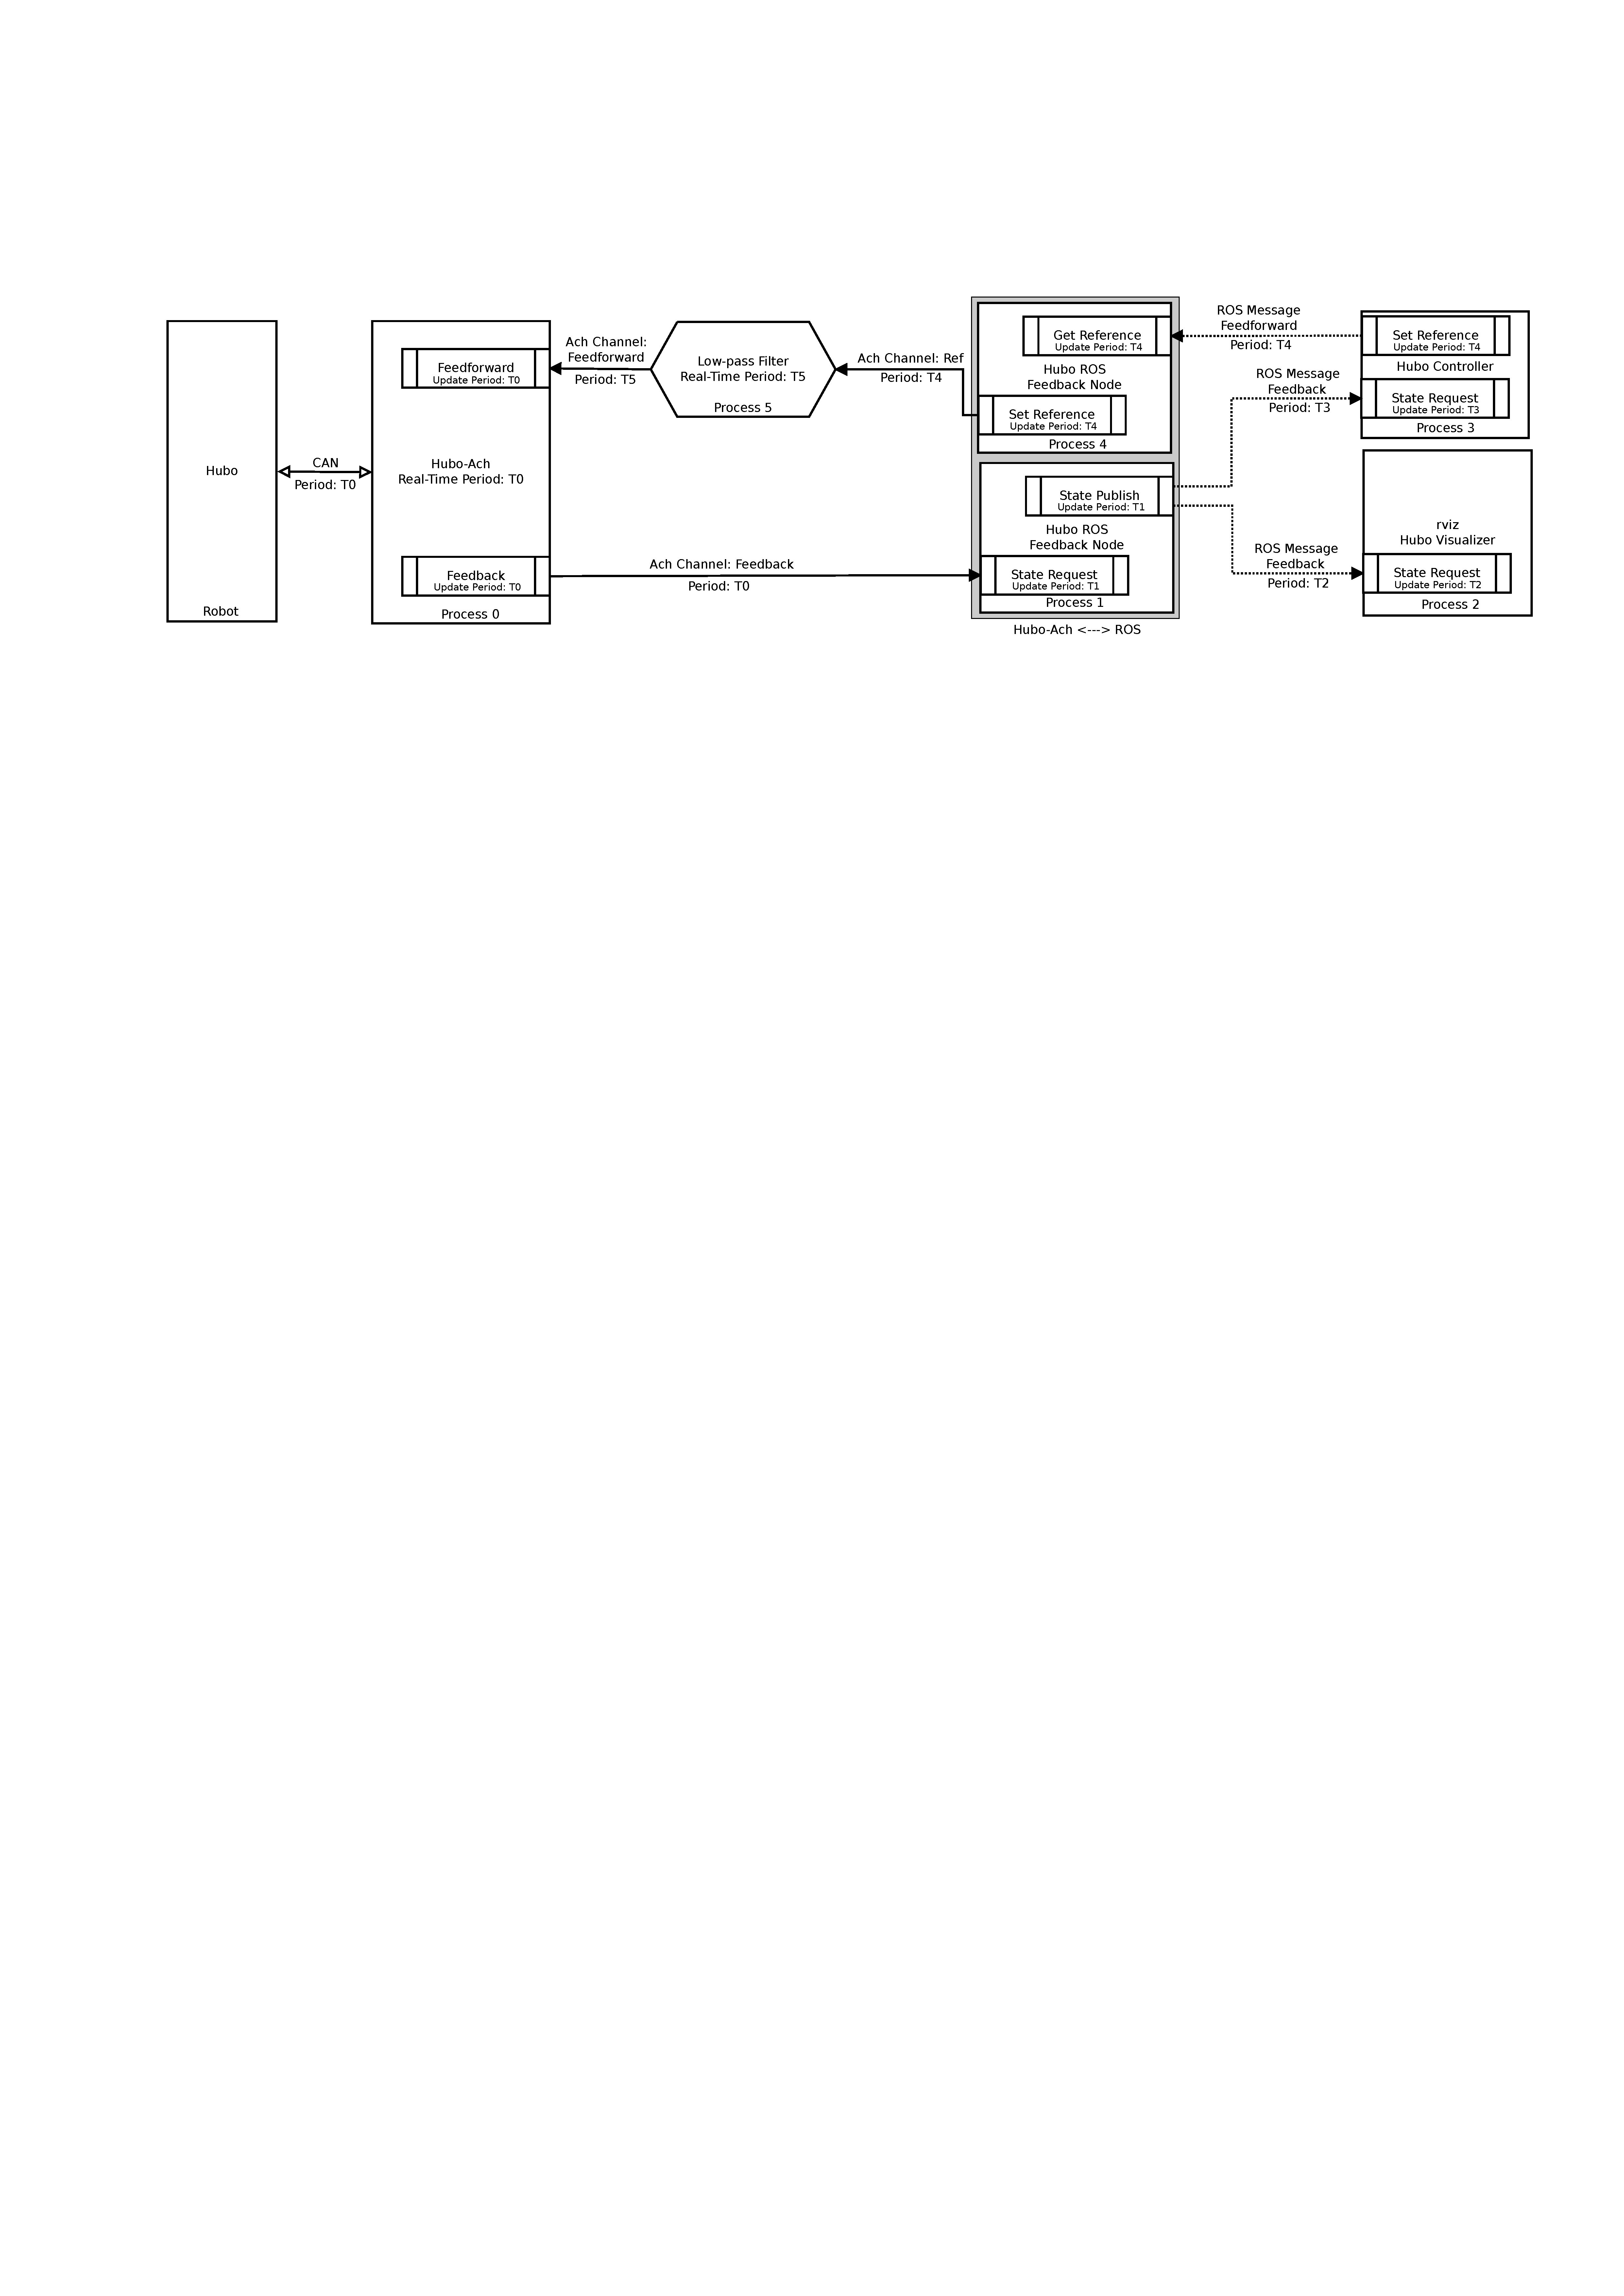
\includegraphics[width=2.0\columnwidth]{./pix/hubo-ach-diagram-ros.pdf}
%   \caption{Hubo-Ach.}
%   \label{fig:graph}
% \end{figure*}
%\definecolor{nodecolor}{RGB}{238,232,170} % light goldenrod
\begin{figure*}
  \centering
  \begin{tikzpicture}
    \node[fill=bgcolor,rounded corners=1em,draw=black,minimum
    width=\textwidth] {
  \begin{tikzpicture}[fill=white, rounded
    corners=0em,draw=black,minimum width=1em]
    \tikzstyle{proc} = [rectangle,minimum height=2.0em,minimum
    width=2.00em, font=\small,draw=black, node distance=72pt,fill=nodecolor]
    \tikzstyle{ros} = [rectangle,minimum height=2.0em,minimum
    width=2.00em, font=\small,draw=black,fill=nodecolor]
    \tikzstyle{ach} =[->, >=stealth,thick,color=black]
    \tikzstyle{ros} =[->, >=stealth,thick,dotted,color=black]
    \tikzstyle{can} =[<->, >=stealth,thick,color=green]
    \tikzstyle{lbl} =[font=\footnotesize,color=black];
    \tikzstyle{keylabel} = [node distance=1.5em]

    \node[proc,,name=achros,xshift=0]{{\tt hubo-ach-ros}};


    \node[proc,right of=achros,name=filter,xshift=0pt]{{\tt filter}};
    \node[proc,right of=filter,name=hubod,xshift=0pt]{{\tt
        hubo-daemon}}; \node[name=hardware,draw=black,right
    of=hubod,xshift=72pt,yshift=-18pt,fill=white]{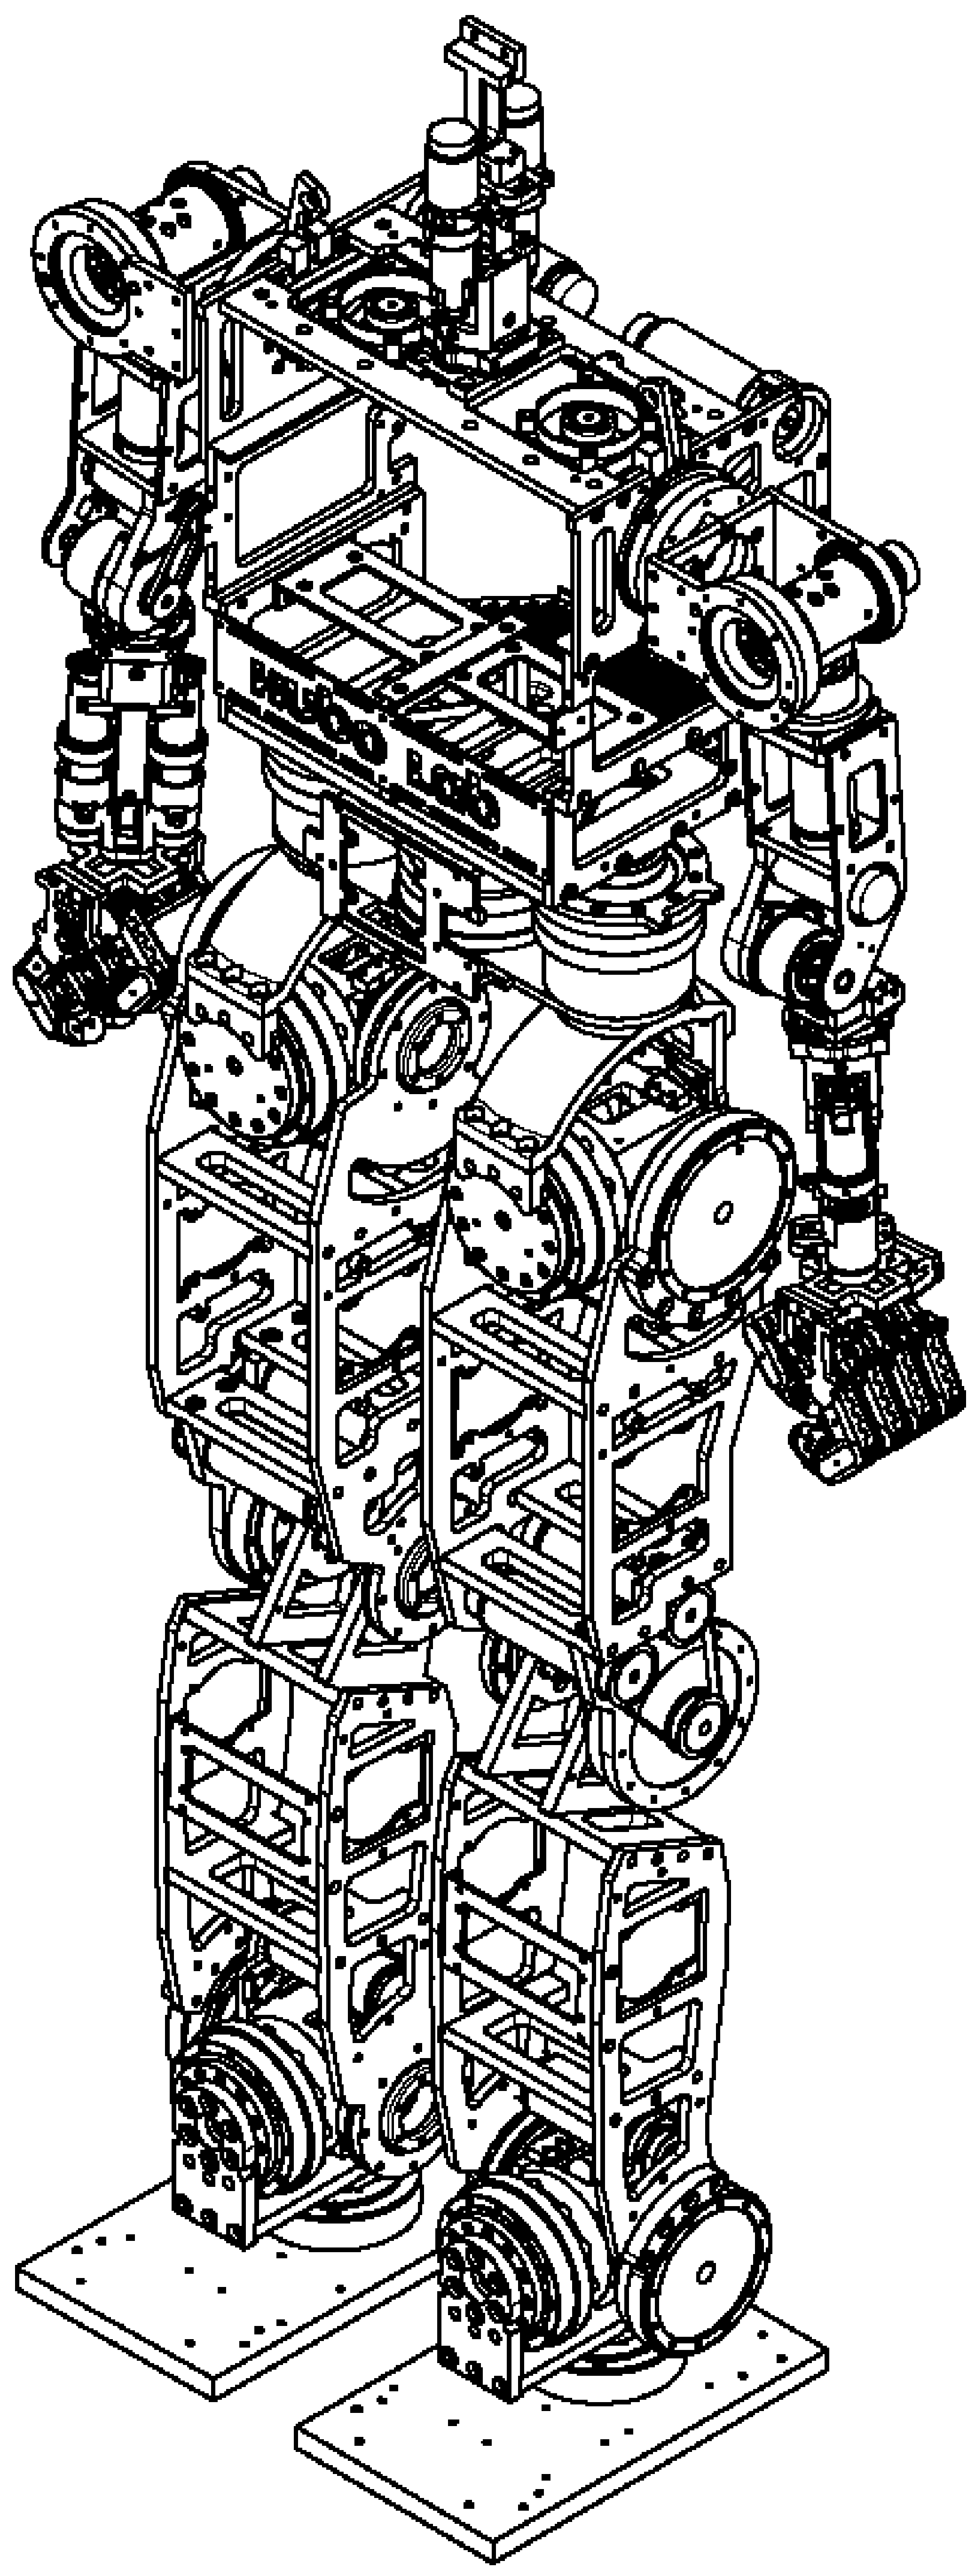
\includegraphics[height=72pt]{pix/hubo-iso}};

    \path(hubod) edge[can] node[above,lbl]{CAN}
    ($(hardware.west)+(0,18pt)$);
    \path (filter) edge[ach] node[above,lbl,yshift=10pt]{\tt feedforward} (hubod);
    \path (achros) edge[ach] node[above,lbl,yshift=10pt]{\tt ref} (filter);

    \draw[thick,->] (hubod) -- ++(0,-36pt) -- node[lbl][above]{\tt
      feedback} ++(-134pt,0)  -- ($(achros.south) + (10pt,0)$) ;

    \node[proc,name=planner,left of=achros,xshift=-36pt] {\tt planner};
    \node[proc,name=rviz,below of=planner,yshift=36pt] {\tt rviz};

    %\draw[ros] ($(achros.south west)$)  -- ($(controller.south east)$);

    \draw[ros] ($(achros.south)+(-10pt,0)$)  --
    ($(rviz)+(72pt,0)+(26pt,0)$) -- node[lbl,above]{\tt rFeedback} (rviz);
    \draw[ros] ($(rviz)+(20.0pt,-.25pt)$) -- ++(0,26pt);

    \path (planner) edge[ros] node[above,lbl,yshift=10pt] {\tt rFeedforward} (achros);


    \node[right of=hardware,name=key,xshift=3em,yshift=36pt] {Key};
    \node[keylabel,below of=key,name=can,xshift=1em] {CAN};
    \node[keylabel,below of=can,name=ach] {Ach};
    \node[keylabel,below of=ach,name=ros] {ROS};

    \path ($(key)+(-24pt,-1.5em)$) edge[can] (can);
    \path ($(key)+(-24pt,-3em)$) edge[ach] (ach);
    \path ($(key)+(-24pt,-4.5em)$) edge[ros] (ros);
  \end{tikzpicture}
  };
  \end{tikzpicture}
  \caption{Feedback loop integrating Hubo-Ach with ROS}
  \label{fig:huboachros}
\end{figure*}


%   It was
% designed by Daniel M. Lofaro\footnote{Daniel M. Lofaro:
%   http://danlofaro.com/} and Neil Dantam in collaboration with the
% \textit{Drexel Autonomous Systems Lab} at Drexel University and
% \textit{Golems - The Humanoid Robotics Laboratory}\footnote{Golems -
%   The Humanoid Robotics Laboratory: www.golems.org/} at the Georgia
% Institute of Technology.

Hubo-Ach \footnote{Available under permissive license,
  \url{http://github.com/hubo/hubo-ach}} is an Ach-based interface to Hubo's
sensors and motor controllers.  This provides a conventional GNU/Linux
programming environment, with the variety of tools available therein,
for developing applications on the Hubo.  It also efficiently links
the embedded electronics and real-time control to popular frameworks
for robotics software: ROS \cite{Quigley09},
OpenRAVE,\footnote{OpenRAVE: http://openrave.org/} and
MATLAB\footnote{MATLAB: http://www.mathworks.com/}.

%  The overarching
% goal of the Hubo-Ach system is to create an easy to use interface
% between the Hubo's electro-mechanical hardware and its programming
% environment.  System design decisions were made with the programmers
% and developers of the Hubo in mind.  This design philosophy
% streamlines closed-loop controller implementation, human robot
% interaction development and the utilization of popular robot related
% systems such as ROS\footnote{ROS: http://www.ros.org/} (Robot
% Operating System), OpenRAVE\footnote{OpenRAVE: http://openrave.org/}
% and MATLAB\footnote{MATLAB: http://www.mathworks.com/} on the Hubo
% platform.

Reliability is a critical issue for software on the Hubo.  As a
bipedal robot, Hubo must constantly maintain dynamic balance; if the
software fails, it will fall and break.  A multi-process software
design improves Hubo's reliability by isolating the critical balance
code from other non-critical functions, such as control of the neck or
arms.  For the high-speed, low-latency communications and priority
access to latest sensor feedback, Ach provides the underlying IPC.

% The inherent complex nature
% and instability of humanoids means the controller is required to be
% active at all times.  Thus the Hubo-Ach system must be immune to
% crashes due to unstable software interfacing with the system.  Our
% solution is to separate Hubo-Ach and the controllers into stand-alone
% processes with the ability to \textit{``talk to each other''} through
% inter process communications also known as IPC.  This allows for one
% or more controllers to crash and not cause Hubo-Ach or other the
% controller processes to fail as well.  Closed-loop control of the Hubo
% requires high-speed, low-latency communications.  Priority access to
% the most recent state data (i.e. sensor feedback) is needed.  The IPC
% called Ach \cite{ach} fit all of the above criteria and thus was used
% for the inter process communications for the Hubo-Ach system.

Hubo-Ach handles CAN bus communication between the PC and embedded
electronics.  Because the motor controllers synchronize to the control
period in a \emph{phase lock loop} (PLL), the single {\tt hubo-daemon}
process runs at a fixed control rate and communicates on the bus.  The
embedded controllers lock to this rate and linearly interpolate
between the commanded positions, providing smoother trajectories in
the face of limited communication bandwidth.  This communication
process also avoids bus saturation; with CAN bandwidth of 1 Mbps and
200Hz control rate, {\tt hubo-daemon} currently utilizes 78\% of the
bus.  {\tt Hubo-daemon} receives position targets from a
{\tt feedforward} channel and publishes sensor data to the
{\tt feedback} channel, providing the direct software interface to
the embedded electronics.

% Hubo-Ach runs as a daemon performing a real-time (RT) loop in the
% background of a Linux based system.  Via the CAN bus the Hubo-Ach
% daemon sets all references to the motor controllers at the rising edge
% of the RT loop then requests the state data from the sensors.  The
% references are taken from the most recently published
% \textbf{Feedforward} Ach channel.  The state data is published to the
% \textbf{Feedback} Ach channel.  All of the data in the
% \textbf{Feedforward} and \textbf{Feedback} Ach channels are in
% \textit{SI} units.  The RT loop runs with a period of $T_0$ which is
% currently set to 5.0 $ms$.  The RT loop in Hubo-Ach is needed to
% ensure the internal phase-locked loop (PLL) of the motor controllers
% lock onto the reference update rate and timing.  Within the motor
% controllers the PLL is used to perform linear interpolation between
% reference commands.  This helps reduce the \textit{jerk} on each of
% the high-gain PID controlled joints.  In addition the RT loop is used
% to ensure the CAN bus's bandwidth is not saturated.  The CAN bus
% bandwidth is 1.0 $Mbps$ and Hubo-Ach currently utilizes is 78\% of it.


Each Hubo-Ach controller is an independent processes.  The controllers
handle tasks such as balance, manipulation, and human-robot
interaction.  Each controller asynchronously reads state from the {\tt
  feedback} Ach channel and sets reference positions in the {\tt
  feedforward} channel.  {\tt Huobo-daemon} reads the most recent
reference position from the {\tt feedforward} channel on the the
rising edge of its control cycle.  This allows the controller
processes to run at arbitrary rates without effecting the PLL of the
embedded motor controllers or the CAN bus bandwidth utilization.


\begin{figure}[thpb]
  \centering
  \begin{tikzpicture}
    %\clip [rounded corners=1em] (0,0) rectangle coordinate (centerpoint) (5,7.5cm);
    \node[minimum width=\linewidth,minimum height=174pt,draw=black,rounded corners=1em,fill=bgcolor,draw=black]
    {};
    \node[name=img] {
      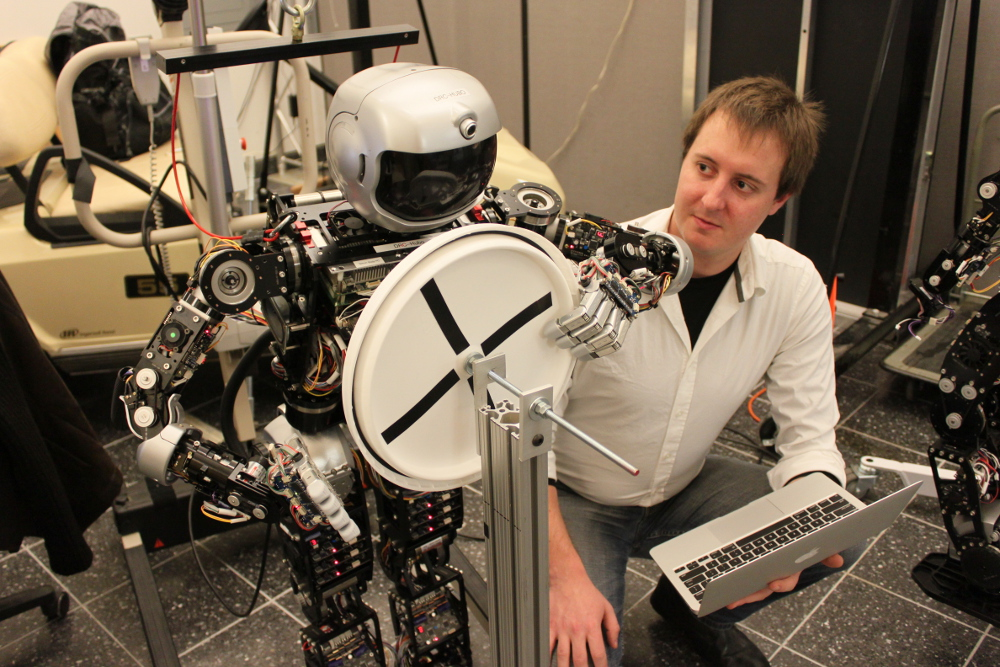
\includegraphics[width=0.93\columnwidth]{./pix/IMG_9107-small.jpg}
    };
    \draw [bgcolor, rounded corners=1em, line width=1em,inner sep=0pt]
    (img.north west) --
    (img.north east) --
    (img.south east) --
    (img.south west) -- cycle
    ;
  \end{tikzpicture}
\caption{Hubo (left) turning a valve via Hubo-Ach alongside Daniel
  M. Lofaro (right).  Valve turning developed in conjunction with
  Dmitry Berenson at WPI for the DARPA Robotics Challenge.}
  \label{fig:valve}
\end{figure}

\autoref{fig:huboachros} shows an example control loop integrating
Hubo-Ach and ROS.  The {\tt hubo-daemon} communicates with the
embedded controllers at $200 \hertz$, publishing to the {\tt feedback}
channel.  The {\tt hubo-ach-ros} process bridges ROS topics and Ach
channels.  It translates messages on the {\tt feedback} Ach channel to
the {\tt rFeedback} ROS topic and translates the {\tt rFeedforward}
ROS topic to the {\tt ref} Ach channel.  The {\tt planner} process
computes desired trajectories, which are relayed via {\tt
  hubo-ach-ros} to {\tt filter} for preprocessing to smooth the motion
and reduce \emph{jerk} before {\tt hubo-daemon} communicates
references to the embedded controllers.  During operation, {\tt rviz}
displays a 3D model of the Hubo's current state.  Each of these
process runs asynchronously, communicating at different rates;
however, {\tt hubo-ach-daemon} maintains its $200 \hertz$ cycle,
ensuring phase lock with the embedded controllers.  This control loop
effectively integrates real-time IPC and control under Hubo-Ach with
the non-real-time ROS environment.

% \textit{Process 2} is the feedforward portion of the
% Hubo-Ach to ROS and ROS to Hubo-Ach bridge.  It reads the
% \textit{aFeedback} channel at given rate and publishes the data to the
% ROS topic \textit{\textbf{Feedback}}.  The data published is the state
% data found in \textbf{aFeedback} at the time it was read.  The rate it
% is read at can be the same or different from that of \textit{Process
%   1} and does not have to be regular.  \textit{Process 2} is a Hubo
% visualizer that reads the state data off of the ROS topic
% \textbf{rFeedback} and applies it to the OpenHUBO model in rviz.
% \textit{Process 3} is the closed loop controller.  It takes in the
% state data from the \textbf{rFeedback} ROS topic, performs a control
% such as visual servoing, impedance control, path-planning etc.  The
% resulting joint space references are published to the
% \textbf{rFeedforward} ROS topic.  \textit{Process 4} is event based
% where when a new message is posted on \textbf{rFeedforward} the second
% part of the Hubo-Ach to ROS and ROS to Hubo-Ach bridge it posts the
% references in the ROS message to the \textbf{aRef} Ach Channel.  To
% allow step inputs to be commanded to the robot without damaging the
% joints a low-pass filter is added between ROS and the Hubo-Ach daemon
% \textit{Process 5}.  This filter reduces the \textit{jerk} on each
% joint.  The resulting filtered reference is posted to the
% \textbf{aFeedforward} Ach channel where the Hubo-Ach daemon can read
% it and command the Hubo.

Hubo-Ach is in use for numerous projects at several research labs.
Users include include groups at MIT, WPI, Ohio State, Purdue,
Swarthmore College, Georgia Tech, and Drexel University.  These
projects primarily revolve around the DARPA Robot Challenge
(DRC)\footnote{DARPA Robot Challenge:
  http://www.theroboticschallenge.org/} team
DRC-Hubo\footnote{DRC-Hubo Homepage: http://drc-hubo.com/}.  The DRC
includes rough terrain walking, ladder climbing, valve turning,
vehicle ingress/egress and more.  \autoref{fig:valve} shows the Hubo
using the Hubo-Ach system to turn a valve.

%   The video of the valve
% turning example can be found at http://drc-hubo/video/valve-example/.

Hubo-Ach provides an effective base for developing real-time
applications on the Hubo.  Separating software modules into different
processes increases system reliability.  A failed process can be
independently restarted, minimizing chance of damage to the robot.  In
addition, the controllers can run at fast rates because Ach provides
high-speed low-latency communication with {\tt hubo-daemon}.  Hubo-Ach
provides a C API that is easily called from high-level programming
languages and integrates with popular platforms for robot software
such as ROS and MATLAB, providing additional development flexibility.
Hubo-Ach is a validated and easy to use interface between the
mechatronics and the software control algorithms of the Hubo full-size
humanoid robot.

% The key point is that Hubo-Ach updates the state data in the
% \textbf{aFeedback} channel and commands the motors with the references
% set in the \textbf{aFeedforward} channel in real-time.

%%% Local Variables:
%%% mode: latex
%%% TeX-master: "ach"
%%% End:


\bibliographystyle{IEEEtran}
%\bibliographystyle{plain}
\bibliography{./hubo-ach.bib,./bibtex.bib}{}




\end{document}
